\subsubsection*{16.a}
Creer utilisateur Test et lui donner tous les droits

\lstinputlisting[style=sqlstyle]{SQL/Partie5/create.sql}

\begin{center}
    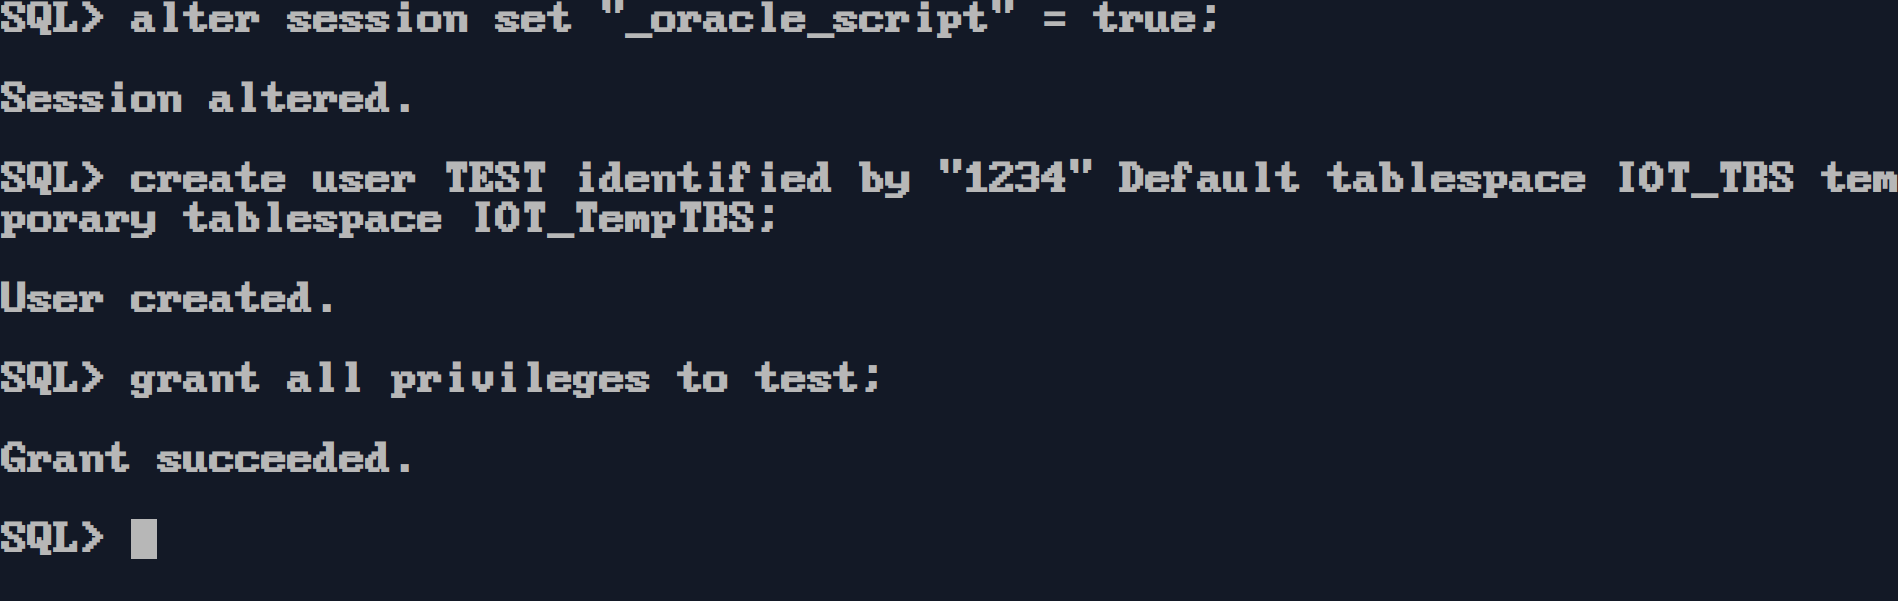
\includegraphics[width=\textwidth]{ScreenShot/Partie5/create.png}
\end{center}

\subsubsection*{16.b}
Connecter en tant que Test

\lstinputlisting[style=sqlstyle]{SQL/Partie5/connecttest.sql}

\begin{center}
    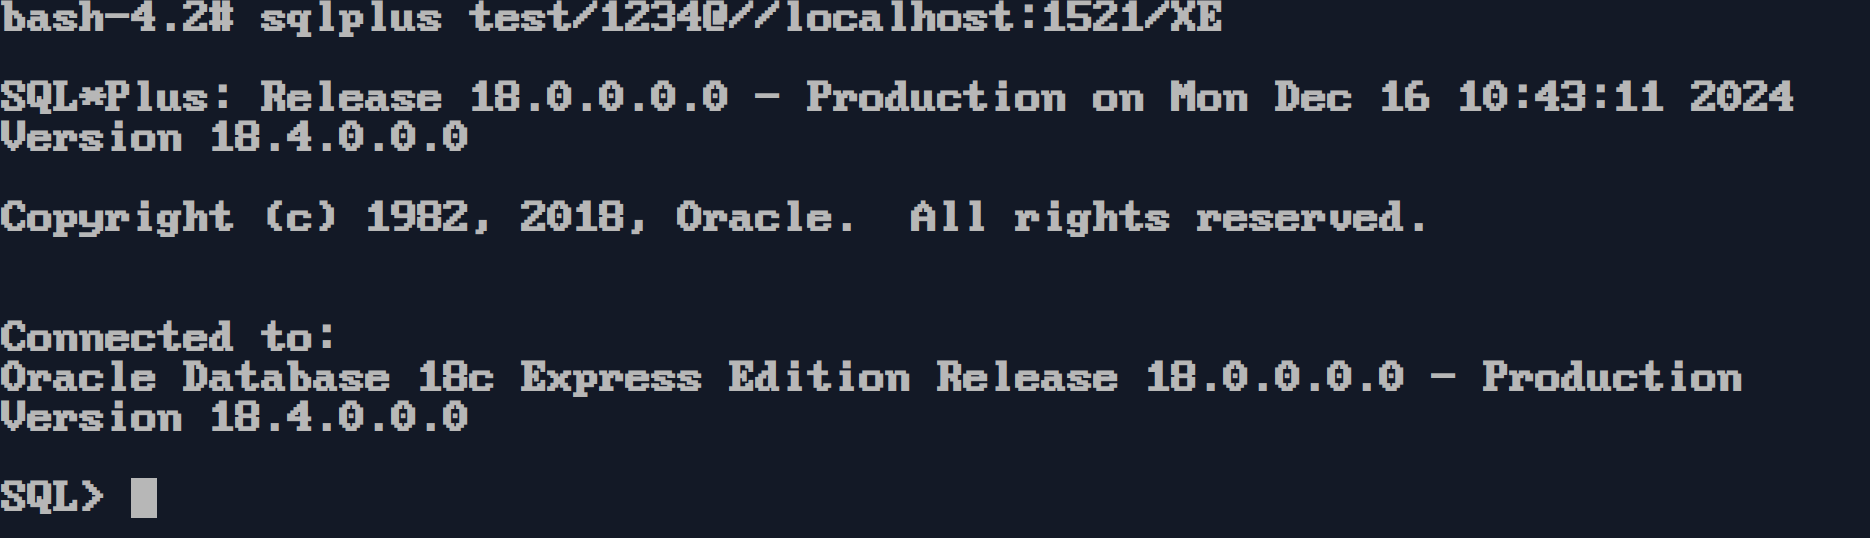
\includegraphics[width=\textwidth]{ScreenShot/Partie5/connecttest.png}
\end{center}

\subsubsection*{16.c}

On va afficher les tables USER\_OBJECTS , USER\_TAB\_COLUMNS , USER\_CONSTRAINTS 
avant et apres des query DDL


\lstinputlisting[style=sqlstyle]{SQL/Partie5/testobj.sql}

\begin{center}
    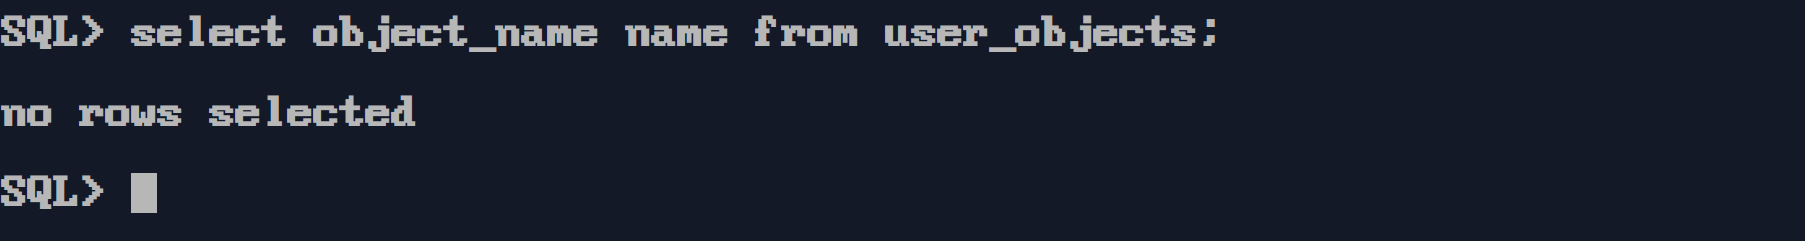
\includegraphics[width=\textwidth]{ScreenShot/Partie5/testobj1.png}
\end{center}


\lstinputlisting[style=sqlstyle]{SQL/Partie5/testatt.sql}

\begin{center}
    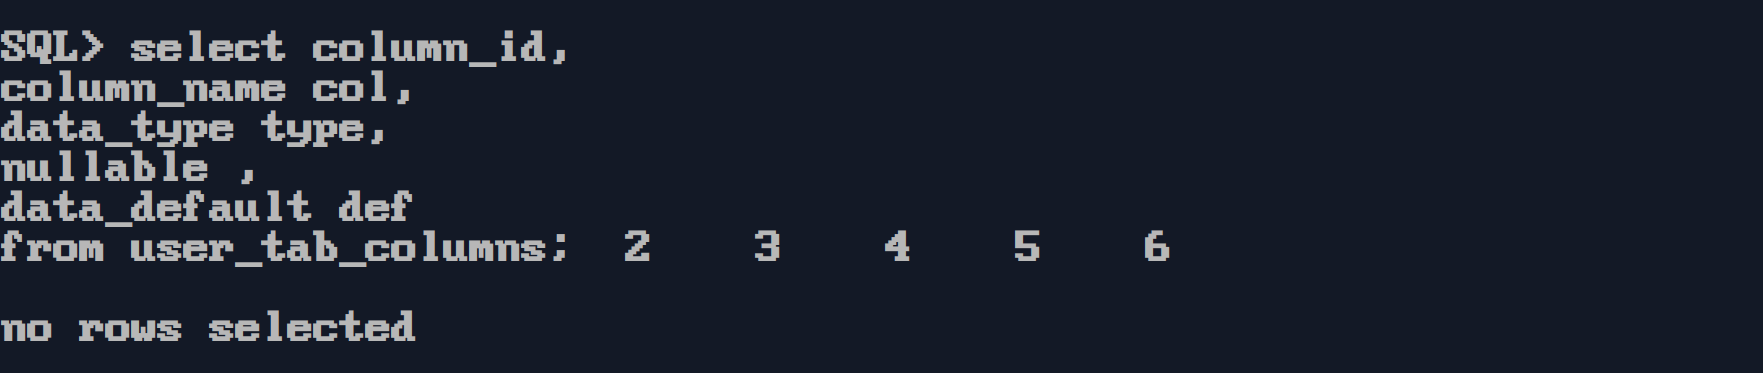
\includegraphics[width=\textwidth]{ScreenShot/Partie5/testatt1.png}
\end{center}


\lstinputlisting[style=sqlstyle]{SQL/Partie5/const.sql}

\begin{center}
    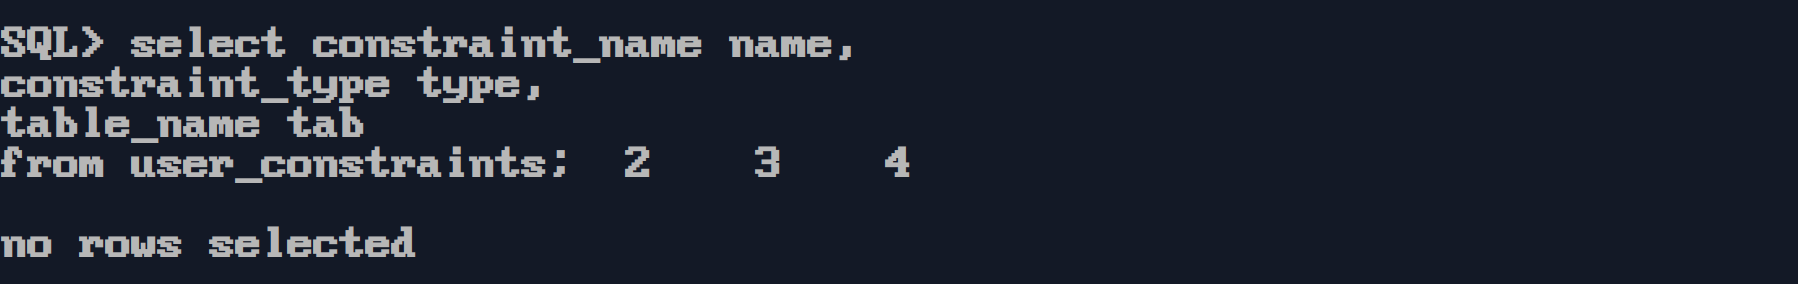
\includegraphics[width=\textwidth]{ScreenShot/Partie5/testconst1.png}
\end{center}

\begin{prettyBox}{Remarque}{myblue}
Puisque test n'a jamais creer de contraints , attribut, objets toute les tables renvoit 0 lignes
\end{prettyBox}

On va creer deux Table t1 et t2

\lstinputlisting[style=sqlstyle]{SQL/Partie5/tab.sql}


\begin{center}
    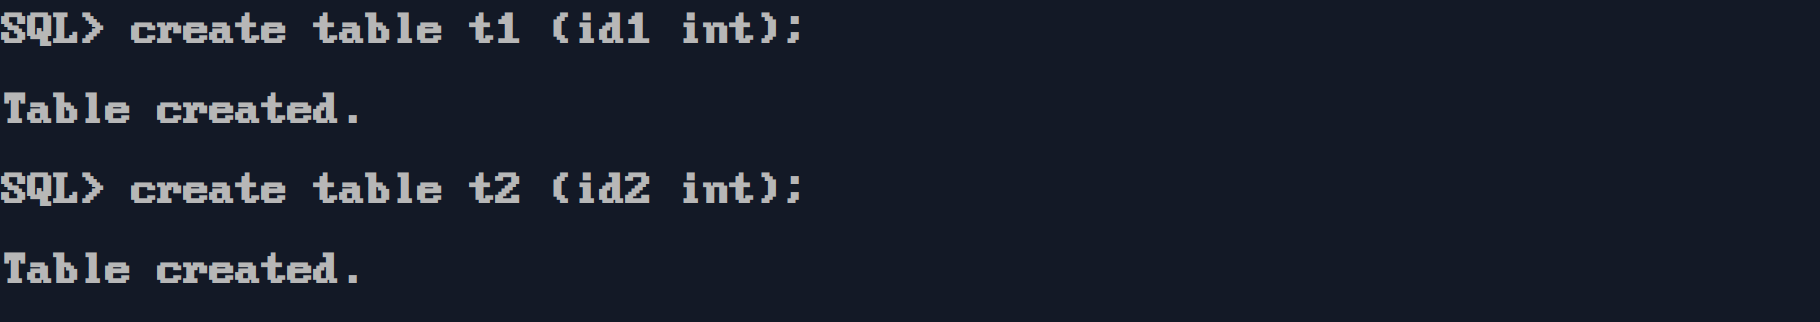
\includegraphics[width=\textwidth]{ScreenShot/Partie5/tab.png}
\end{center}


On va afficher les object et attribut de Test
\lstinputlisting[style=sqlstyle]{SQL/Partie5/testobj.sql}

\begin{center}
    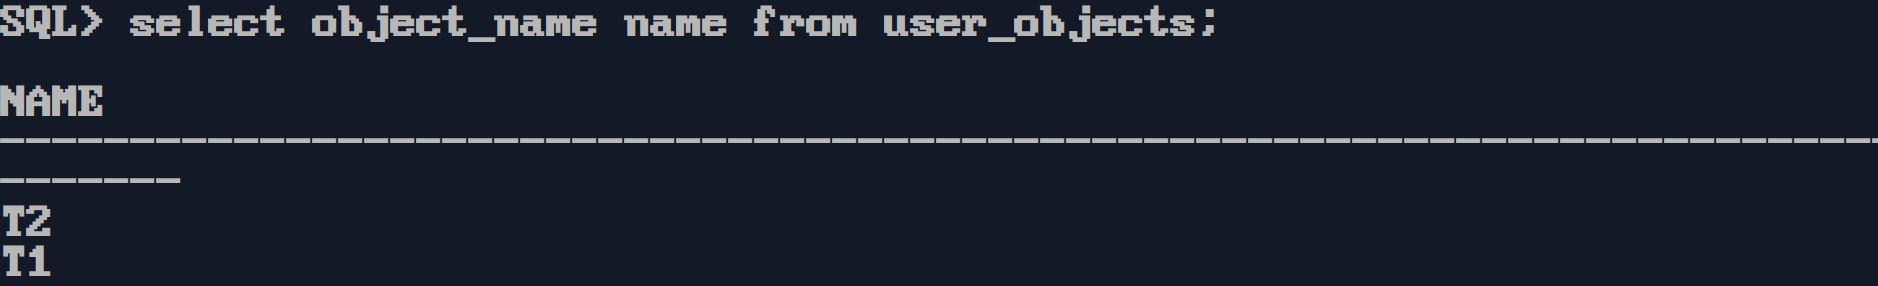
\includegraphics[width=\textwidth]{ScreenShot/Partie5/testobj2.png}
\end{center}


\lstinputlisting[style=sqlstyle]{SQL/Partie5/testatt.sql}

\begin{center}
    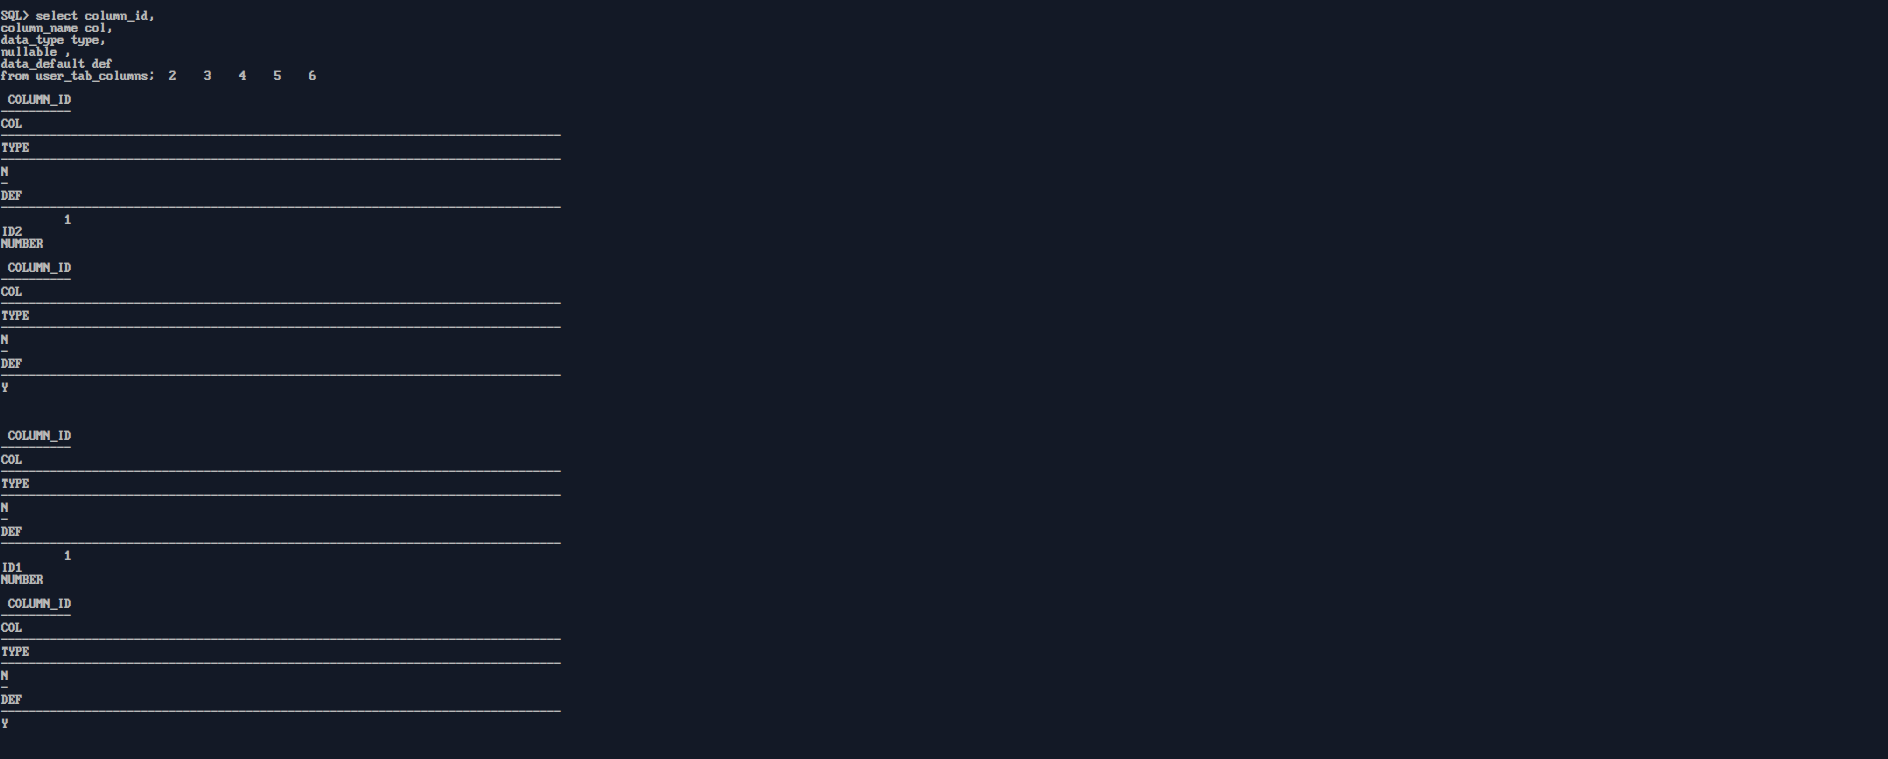
\includegraphics[width=\textwidth]{ScreenShot/Partie5/testatt2.png}
\end{center}

\begin{prettyBox}{Remarque}{myblue}
On remarque apres la creation des deux tables , les tables USER\_OBJECTS , USER\_TAB\_COLUMNS on ete mise a jour
\end{prettyBox}

\vspace{0.25cm}
On va ajouter une colonne a t1 puis afficher les attributes de Test

\lstinputlisting[style=sqlstyle]{SQL/Partie5/col.sql}

\begin{center}
    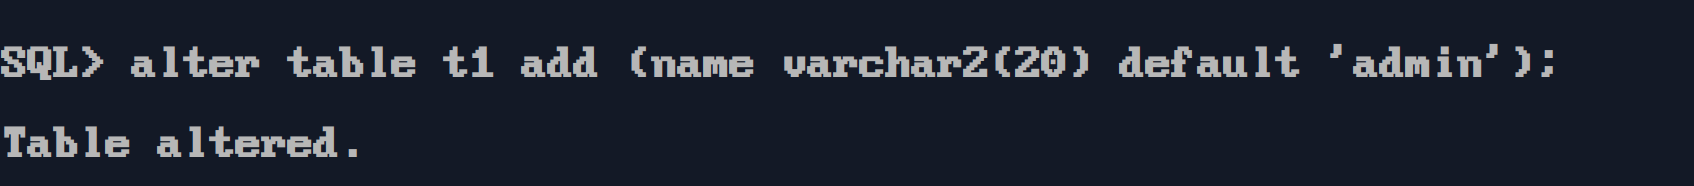
\includegraphics[width=\textwidth]{ScreenShot/Partie5/col.png}
\end{center}

\lstinputlisting[style=sqlstyle]{SQL/Partie5/testatt.sql}

\begin{center}
    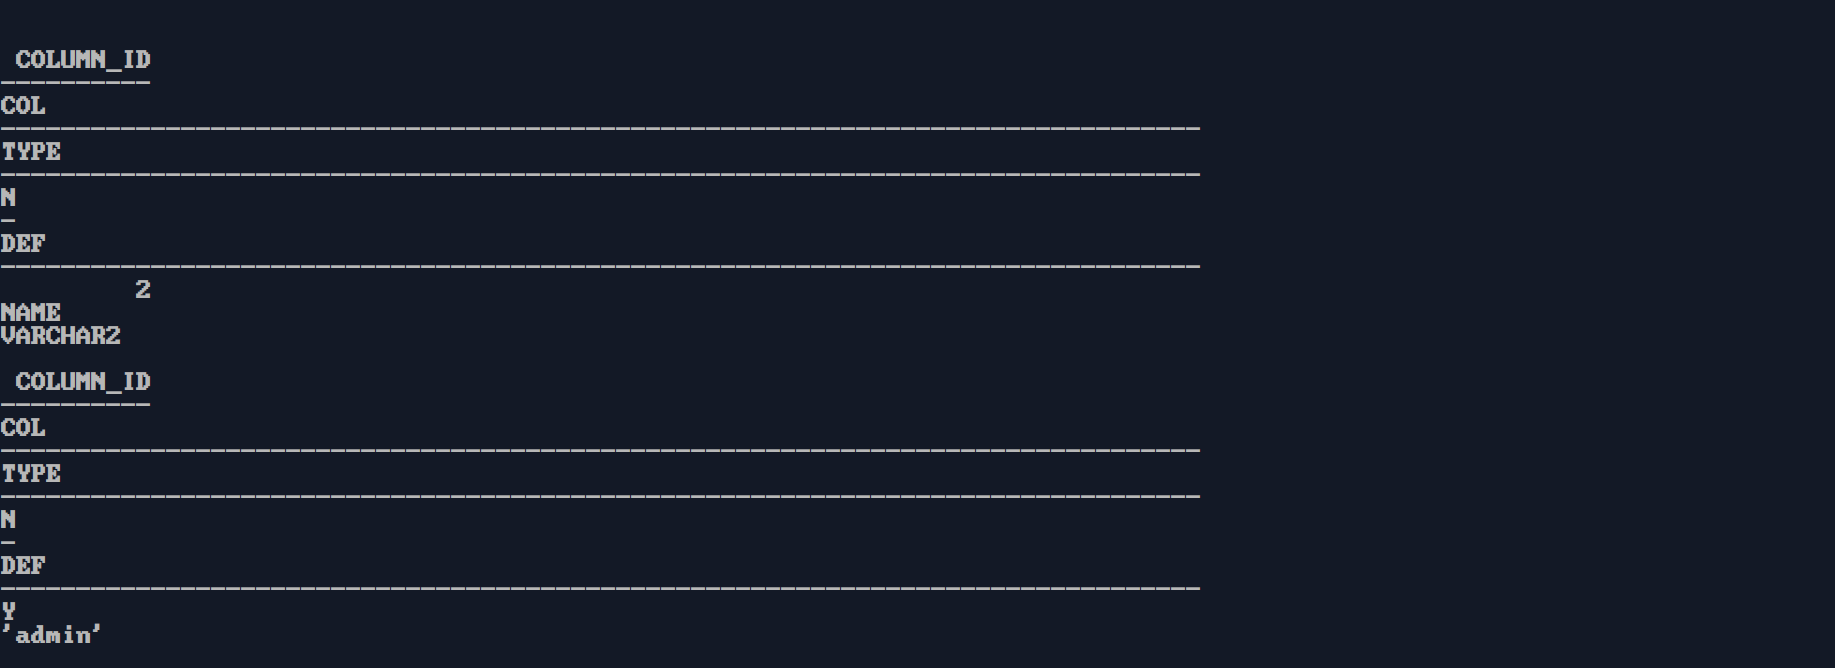
\includegraphics[width=\textwidth]{ScreenShot/Partie5/testatt3.png}
\end{center}

\begin{prettyBox}{Remarque}{myblue}
On appercoie que l'attribut name a ete ajoute a la table USER\_TAB\_COLUMNS et avec sa valeur par defaut 'admin'
\end{prettyBox}

\vspace{0.25cm}
On va ajouter une contraint de cle primaire pour t1 et une unique pour t2
\lstinputlisting[style=sqlstyle]{SQL/Partie5/con.sql}

\begin{center}
    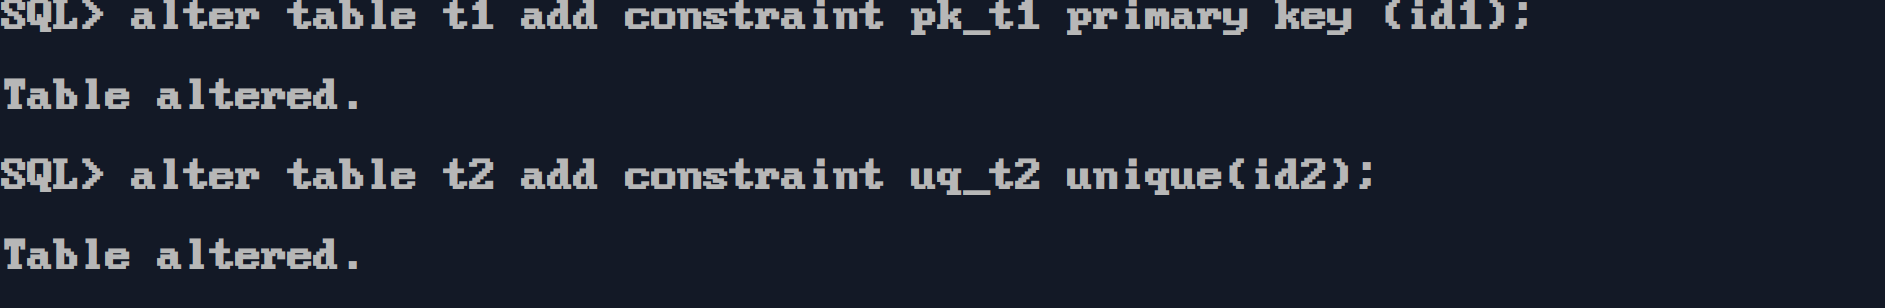
\includegraphics[width=\textwidth]{ScreenShot/Partie5/con.png}
\end{center}

\lstinputlisting[style=sqlstyle]{SQL/Partie5/testatt.sql}

\begin{center}
    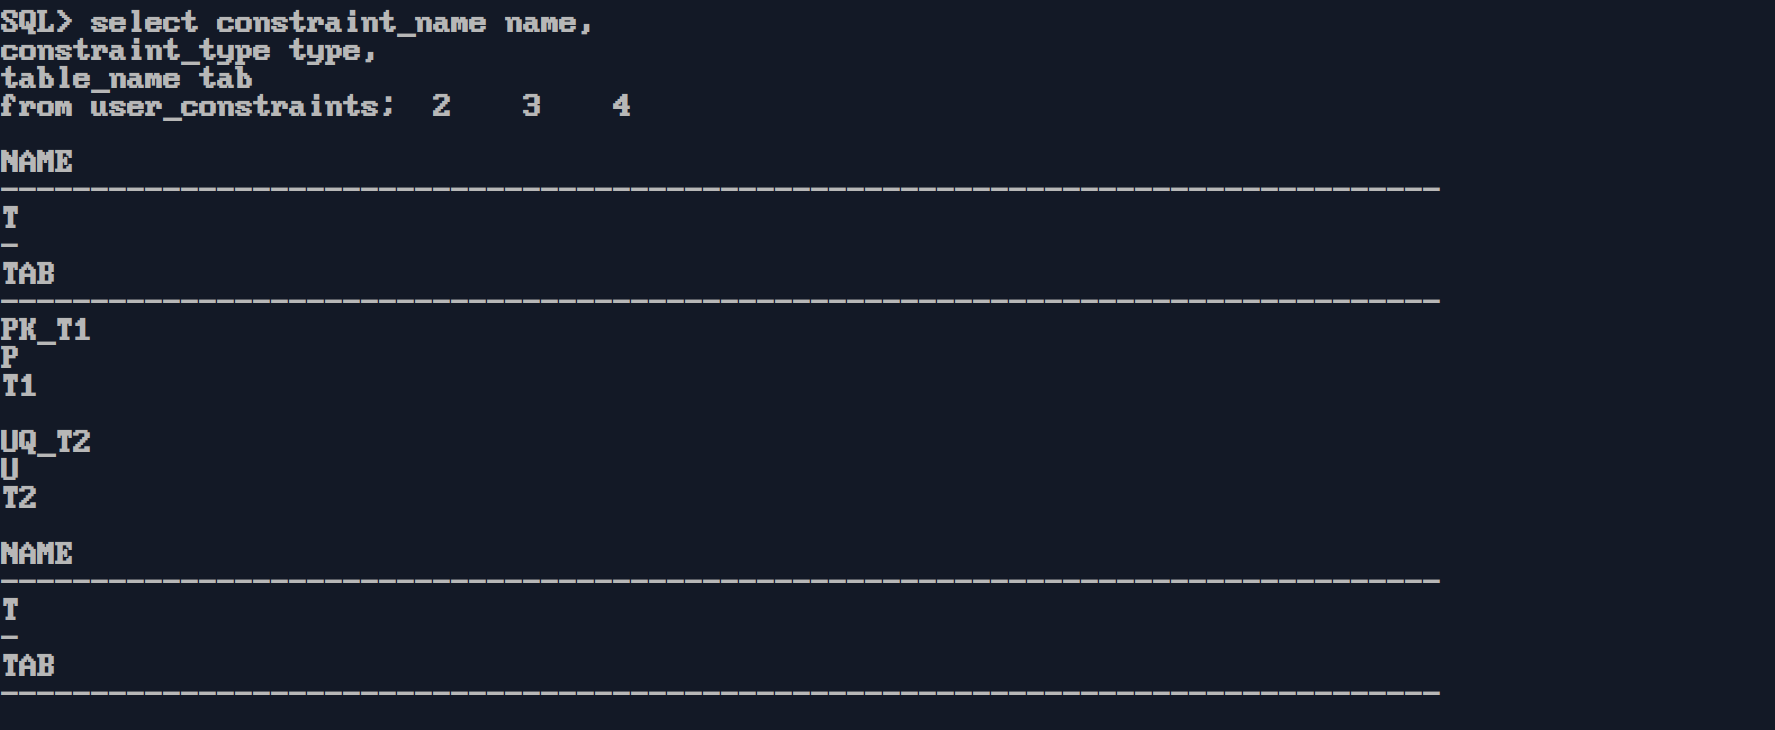
\includegraphics[width=\textwidth]{ScreenShot/Partie5/testconst2.png}
\end{center}

\begin{prettyBox}{Remarque}{myblue}
On remarque qu'apres avoir ajouter les contraintes la table USER\_CONSTRAINTS a ete misajour
\end{prettyBox}




